\documentclass[11pt]{article}

\usepackage[utf8]{inputenc}
\usepackage[left=1in,right=1in]{geometry}
%\usepackage[a4paper,bindingoffset=0.2in,left=1in,right=1in,top=1in,bottom=1in,footskip=.25in]{geometry}
\usepackage[english]{babel}
\usepackage{tocloft}
\usepackage{amsmath}
\usepackage{amsfonts}
\usepackage{amssymb}
\usepackage[none]{hyphenat}
\usepackage{graphicx}
\usepackage{fancyhdr}
\usepackage{pdfpages}
%\usepackage{setspace}
%\usepackage{tikz}
\usepackage[font={small,it}]{caption}


\parindent 0ex
\linespread{1.5}
\setlength{\headheight}{30pt}
\setcounter{tocdepth}{1}
\pagestyle{fancy}

\fancyhead{}
%\fancyfoot{}
\fancyhead[L]{\slshape \MakeUppercase{Binarization of Handwritten Minutes of the Early \newline Synod Meetings of Reformed Churches in South-Africa}}
\rhead{
\includegraphics[width=3.7cm, height=1.2cm]{nwulogo.jpeg}}

\begin{document}
	%insert pdf cover page
	
\includepdf[pages={-},offset=0mm 0mm, width=21.5cm, height=28cm]{Cover.pdf}

    \renewcommand{\cftsecleader}{\cftdotfill{\cftdotsep}} % TOC Dotted Lines
    \tableofcontents
    \thispagestyle{empty}
    \clearpage

    \listoffigures
    \thispagestyle{empty}
    \clearpage

    \setcounter{page}{1}

	\section{Introduction}
		This literature study forms part of the B.Sc. Honours project titled as binarization of handwritten minutes of the early synod meetings of Reformed Churches in South-Africa. All literature researched and reviewed will be discussed in this document. The aim of this study is to propose a binarization algorithm that bests differentiate the foreground (text, tables and figures) from the background (paper and stains) in historical handwritten documentation, specifically on the dataset which is the minutes of the early synod meetings of the Reformed Churches in South-Africa.\\

		A considerable number of binarization algorithms exist and they all have their advantages and disadvantages; some fit better for certain circumstances or for a certain type of image. There exist no binaroization algorithm yet that suits all types of images \cite{lins2015binarizing}, but one can improve the result by combining algorithms \cite{ntogas2008binarization}, by adding pre-processing and post-processing techniques to the binarization algorithm such as noise removal \cite{agrawal2011stroke}, \cite{lins2015binarizing}, or by careful experimentation and analysis on a very specific dataset in order to train the algorithm accordingly. One of the key objectives in binarization is thresholding, which is the calculation algorithm of the middle or ``split'' value used to discriminate the foreground from the background in the image. The algorithm would mark the pixels in a binary fashion and divide them into two categories, ON denoting the set of pixels representing the foreground or OFF denoting the set of pixels representing the background \cite{o1995document}.\\

		This document starts with a literature study on pre-processing techniques used to prepare the document for optimal binarization. Pre-processing techniques is then followed by binarization algorithms and the combination thereof which is followed by post-processing techniques used to enhance and refine the result. Finally the literature study will conclude with evaluation techniques used to determine the successfulness of this project.

	\section{Pre-processing Techniques}
		Some pre-processing techniques such as cropping, deskewing and grey scale transformations which are used to prepare the image for binarization in order to improve binarization efficeiency will be discussed in this section. Other pre-processing techniques includes low pass filters which are good for noise removal, high pass filters which are good for contrast enhancement in order to better diferentiate between foreground pixels and background pixels and gamma correction algorithms which are good for unevenly distributed intensity values \cite{soua2015improved}.

		\subsection{Geometric Corrections}
			The geometric corrections that'll be necessary to prepare the document image for effective \sloppy binarization will mostly consist of cropping and a de-skewing process. Cropping will be necessary to exclude some unnecessary parts of the image which can be found surrounding the information relevant to the document image. This will result in increased binarization performance since the document image would be smaller, this will also result in a lower probability of error or inaccurate binarization since there would be less defective area for the binarization algorithm to take in account. The de-skewing process aims to correct the shape of the document image to a more rectangular shape, it would be perfect if the horizontal margins and the vertical margins are perpendicular.%Kyk na defective

		\subsection{Grey-scale Transformation}
			To simplify the binarization, the document images will undergo a grey-scale transformation. This transformation takes in a colour image and map the three red, green and blue colour scales to a single grey colour scale. It is uncertain whether the grey-scale transformation will be implemented before or after the geometric correction phase, but this will be experimented with to see whether the geometric corrections provide better results with red, green and blue colour scales or with grey colour scales.

		\subsection{Noise Removal} %Wiener filter, homomorphic filter, gamma correction ideal filter, butterwoorth filter,gaussian filter
			De-noising is the process of avergaing the pixel intensitities so one can hide the outlier pixel intensities which is seen as noise, thus some detail in the image may be lost \cite{buades2005non}. A non-local noise removal scheme that has proved itself can be implemented in the pre-processing phase of document binarization \cite{chen2017broken}. A noisy image can be defined as \textit{equation \ref{eq:noise}} where $v(i)$ is the observed image containing noise, $u(i)$ the true image containing no noise and $n(i)$ the noise component at pixel $i$ \cite{buades2005non}. \textit{Figure \ref{fig:denoise}} shows an example of what the result might look like if the de-noising objectives forms part of the pre-processing phase. One can see some loss in contrast in the de-noised image which could cause a decrease in accuracy during binarization but this can be dealt with since the detail is not completely lost.

		\begin{large}
		\begin{equation} \label{eq:noise}
		v(i) = u(i) + n(i)
		\end{equation}
		\end{large}

		\begin{figure}[!htb]
		 \centering
		 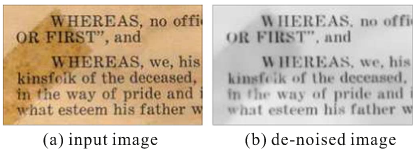
\includegraphics[scale=1]{denoise.png}
		 \caption{De-noising example as explained in \cite{chen2017broken} by Chen \& Wang. (a) Original document image. (b) de-noised image} % Figuur Naam
		 \label{fig:denoise} % label om na figuur te verwys
		\end{figure}

			Low pass filters that are applied to the pre-processing phase proves to provide very good binarization results such as the Wiener, median, butterworth, ideal low pass, and Gaussian filters. These pre-processing filters can reduce effects such as non-uniform distributed intensities(shadows), wrinkles caused by humidity, poor contrast between foreground and background, broken characters in thin ink strokes, bleedthrough and dark dirt spots on the document itself \cite{ntogas2008binarization}. Gatos's binarization algorithm also incorporates noise removal into its pre-processing phase but will be discussed in more detail in \textit{section 3.5}. \\

			Another approach to noise removal is by using the Discrete Cosine Transform prior to binarization, followed by binarizing the transformed image rather than the image in original form, Arnia et al. \cite{arnia2014improvement} shows that this pre-processing techniques may be a good alternative to traditional noise removal algorithms. The Discrete Cosine Transform is defined in \textit{equation \ref{eq:dct}}. Where $f(x, y)$ denotes the original image, and $F(\hat{x}, \hat{y})$ the Discrete Cosine Transform coefficiant and $C(\hat{x})$ the gain control which is defined in \textit{equation \ref{eq:gainC}} \cite{arnia2014improvement}.

			\begin{large}
			\begin{equation} \label{eq:dct}
				F_c(\hat{x},\hat{y}) = \frac{2}{N} C(\hat{x})C(\hat{y})\sum_{x}\sum_{y}f(x, y) \cdot \cos(\frac{(2x + 1)\hat{x}\pi}{2X}) \cdot \cos(\frac{(y + 1) \hat{y} \pi}{2Y})
			\end{equation}
			\end{large}

			\begin{Large}
			\begin{equation} \label{eq:gainC}
			 C(\hat{x}) =
			 \begin{cases}
				\frac{1}{\sqrt{2}},          & \text{if } \hat{x} = 0     \\
				1, & \text{if } \hat{x} \neq 0 \\
			 \end{cases}
			\end{equation}
			\end{Large}

			The Inverse Discrete Cosine Transform is defined in \textit{equation \ref{eq:idct}} which results in an image with a limited frequency band. Where $\hat{f}_c(x,y)$ is the spatial image reproduced from the Discrete Cosine Transformation $\hat{F}_c(\hat{x}, \hat{y})$, in both the forward and backward transformations the $X$ and $Y$ denotes the width and height of the image respectively \cite{arnia2014improvement}.

			\begin{large}
			\begin{equation} \label{eq:idct}
				\hat{f}_c(x,y) = \frac{2}{N} \sum_{\hat{x}}\sum_{\hat{y}} C(\hat{x})C(\hat{y})\hat{F}(\hat{x}, \hat{y}) \cdot \cos(\frac{(2\hat{x} + 1)x\pi}{2X}) \cdot \cos(\frac{(\hat{y} + 1) y \pi}{2Y})
			\end{equation}
			\end{large}

			As demonstrated by Ntogas and Ventzas \cite{ntogas2008binarization} pre-processing does not improve the results for all binarization algorithms but provide some aid to some of the algorithms, which is why the binarization algorithms will be chosen carefully and experimentation with combining them will also be investigated thoroughly while implementing pre-processing techniques.

    \section{Binarization Algorithms}% log based
			After the document image has been pre-processed to be in a geometric shape as close to a perfect document as possible, it will be binarized to differentiate the foreground, meaning text, from the background, meaning the paper. The algorithms used to binarize an image will be inspected and discussed in this section.\\

  		Binarization in image processing is the process of discriminating the foreground from the background in an image by changing the foreground pixels or text to black and the background or paper pixels to white \cite{ntogas2008binarization}. Binarization is also considered by many computer scientists as a critical step in the processing of images because it has the greatest impact on the quality grade of all the processing that follows such as document analysis \cite{jacob2014survey}, thus a good binarization result would greatly improve the results of page-segmentation, optical character recognition and any other subsequent processing \cite{agrawal2011stroke}, while a bad binarization result will cause any following processing techniques to yield inadequate results \cite{howe2011laplacian}. A good binarization algorithm is one that best preserves the foreground and omit as much background as possible.

			\subsection{Local vs. Global Thresholding}
				Thresholding is the process of determining a value that will divide the foreground and backgound, making this calculation a crucial objective to binarization. Global thresholding calculates a value by using the whole document image pixels, this method does not generate as much backgound noise but struggle to keep connectivity in thin stroke lines. Local adaptive binarization uses only a local window of surrounding pixels to calcultae a new threshold value for each pixel which is adapted spesifically for that pixel. this method is better for document images with non-uniform distributed intensity values and does not generate as much noise \cite{chen2017broken}.

			\subsection{Rosenfeld's Threshold Calculation}
				Rosenfeld's method \cite{chen2017broken} for calculating the threshold value $T$ analyzes the concavities of the historgram compared with its convex hull as seen in the log sigmoid \textit{equation \ref{eq:rosenfeld}} \cite{chen2017broken} where $I(x,y)$ denotes the original image, $\delta$ the average difference in the white and black pixels, $c_1$ and $c_2$ the constant parameters with values $c_1=0.5$ and $c_2=0.8$ and $w$ a weighting parameter with value $w=0.6$ as suggested by Chen \& Wang  \cite{chen2017broken}. \textit{Figure \ref{fig:rosenfeld}} shows the result of the binarization by using Rosenfeld's method for calculating a threshold value. This method shows positive results for document images with lack of connectivity among characters as one would find in our document image dataset containing many areas where thin lines of ink strokes are disconnected due to the rapid movements of fountain pens as illustrated in \textit{figures \ref{fig:stroke}} and \textit{\ref{fig:stroke2}}.

				\begin{Large}
				\begin{equation} \label{eq:rosenfeld}
				T(I(x,y)) = w \delta (\frac{(1 - c_2)}{1 + \exp(\frac{-4I(x, y)}{b(1 - c_1)} + \frac{2(1 + c_1)}{(1 - c_1)})} + c_2)
				\end{equation}
				\end{Large}

				\begin{figure}[!htb]
				 \centering
				 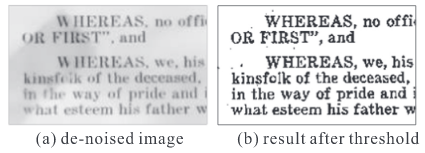
\includegraphics[scale=1]{rosenfeld.png}
				 \caption{Binarization result by using Rosenfeld's method for calculating a threshold value \cite{chen2017broken}. (a) De-noised document image. (b) binarized image} % Figuur Naam
				 \label{fig:rosenfeld} % label om na figuur te verwys
				\end{figure}

				\begin{figure}[!htb]
				 \centering
				 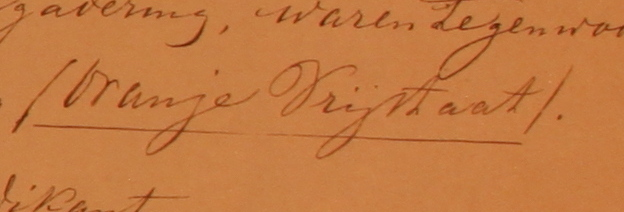
\includegraphics[scale=0.4]{stroke.JPG}
				 \caption{Underlining fountain pen stroke disconnected due to fast movement when writing.} % Figuur Naam
				 \label{fig:stroke} % label om na figuur te verwys
				\end{figure}

				\begin{figure}[!htb]
				 \centering
				 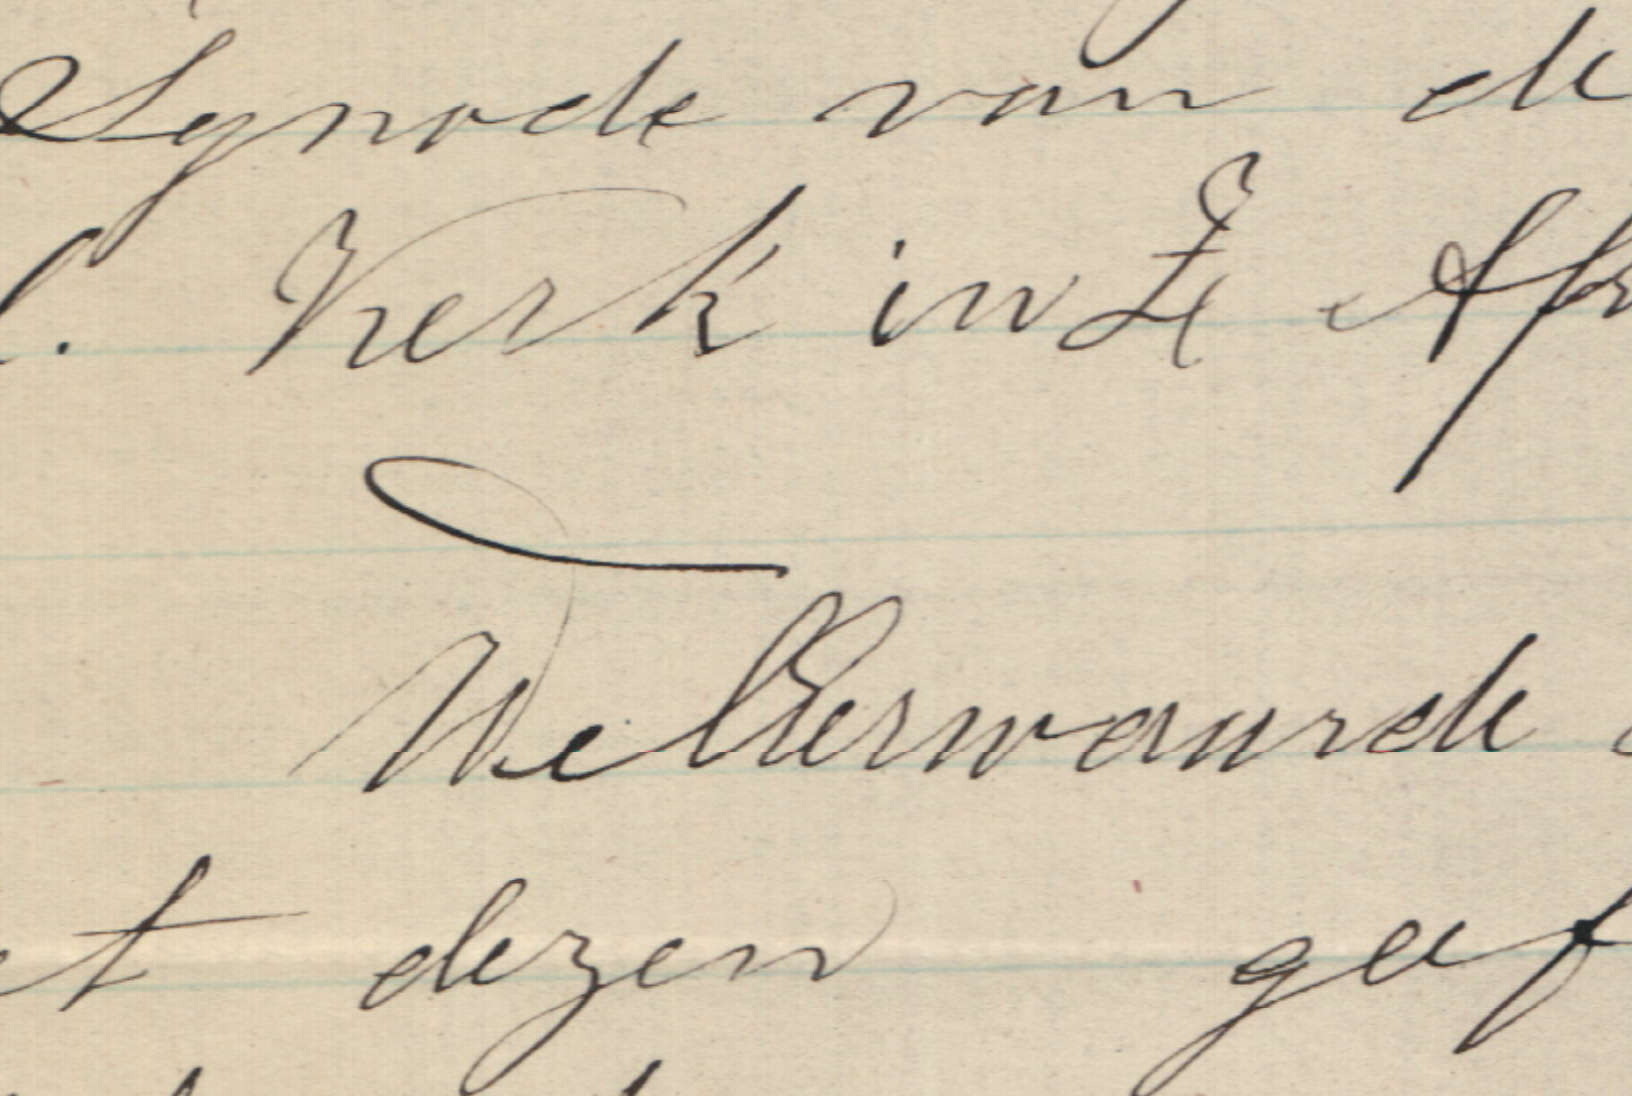
\includegraphics[scale=1]{stroke2.JPG}
				 \caption{Letters with broken ink strokes.} % Figuur Naam
				 \label{fig:stroke2} % label om na figuur te verwys
				\end{figure}

				%Otsu?
				\newpage

  		\subsection{Niblack Algorithm}% vertel storie van eerste algo ens.
  			The Niblack algorithm \cite{niblack1985introduction} calculates a local threshold by using the mean and the standard deviation of all the pixels in the local neighbourhood window. This method is good at classifying text as foreground but produces background noise. \textit{Equation \ref{eq:niblack}} shows the calculation of the threshold value for the Niblack binarization algorithm where $m(I(x, y))$ denotes the mean of the pixel intensity values of all the pixels inside of the local window which contains the pixel $(x, y)$ in image $I$, $k$ a constant value of $-0.2$ as suggested by Khurshid et al. \cite{khurshid2009comparison} and $S(I(x, y))$ the standard deviation of the pixel intensities of the complete image \cite{khurshid2009comparison}.

				\begin{large}
				\begin{equation} \label{eq:niblack}
					T(I(x, y)) = m(I(x, y)) + k \cdot S(I(x, y))
				\end{equation}
				\end{large}

				\newpage

				The mean of the local window is calculated in \textit{equation \ref{eq:niblack_mean}} where $floor(x)$ rounds the value of $x$ down to the closest integer less than $x$, and $X$ denotes the local window size in the horizontal dimension and $Y$ in the vertical dimension \cite{khurshid2009comparison}.

				\begin{large}
				\begin{equation} \label{eq:niblack_mean}
					m(I(x, y)) = \sum_{i = floor(\frac{-Y}{2})}^{i < floor(\frac{Y}{2})}\sum_{j = floor(\frac{-X}{2})}^{j < floor(\frac{X}{2})} I(x + j, y + i)
				\end{equation}
				\end{large}

				The standard of the entire image is calculated in \textit{equation \ref{eq:niblack_S}} where $N$ and $M$ denotes the size of the entire image in the horizontal and vertical dimensions respectively and $M(I(x, y))$ the mean of the pixel intensities of the entire image \cite{khurshid2009comparison}.

				\begin{large}
				\begin{equation} \label{eq:niblack_S}
					S(I(x, y)) = \sqrt{\frac{1}{NM} \sum_{i = 1}^{i \leq N}\sum_{j = 1}^{j \leq M}(I(i, j) - M(I(x, y)))^2}
				\end{equation}
				\end{large}

				The mean of the pixel intensities of the entire image is calculated in \textit{equation \ref{eq:niblack_M}} where $X$ and $Y$ denotes the size of the entire image in the horizontal and vertical dimensions respectively.

				\begin{large}
				\begin{equation} \label{eq:niblack_M}
					M(I(x, y)) = \sum_{i = 1}^{i \leq X}\sum_{j = 1}^{j \leq Y} I(i, y)
				\end{equation}
				\end{large}

  		\subsection{Sauvola's Algorithm}
  			Sauvola's algorithm \cite{sauvola1997adaptive} calculates the threshold value by using the standard deviation of the image's dynamic range. This method is an improvement over the Niblack algorithm in high contrast images so it provides inadequate results when the contrast between the foreground and background decreases. \textit{Equation \ref{eq:sauvola}} shows the calculation of the threshold value for Sauvola's binarization algorithm where $k$ and $R$ are constants set to $0.5$ and $128$, respectively, as suggested by Khurshid et al. \cite{khurshid2009comparison}, $m(I(x, y))$ calculates the mean of the pixel intensities in the local window as seen in \textit{equation \ref{eq:niblack_mean}}, and $S(I(x, y))$ the standard deviation of all the pixels in the entire image as seen in \textit{equation \ref{eq:niblack_S}} \cite{khurshid2009comparison}.

				\begin{large}
				\begin{equation} \label{eq:sauvola}
					T(I(x, y)) = m(I(x, y)) \cdot (1 - k \cdot (1 - \frac{S(I(x, y))}{R}))
				\end{equation}
				\end{large}

			\subsection{Gatos' Algorithm}
				Gatos combined existing algorithms \cite{gatos2006adaptive}, his method uses a Wiener filter in a pre-processing phase to eliminate noise and to enhance the contrast of the image before binarization takes place. \textit{Equation \ref{eq:gatos_pre-processing}} shows how the image is pre-processed. $I_{pre}(x,y)$ denotes the image after pre-processing and $I(x,y)$ the original gray scale image. $\mu$ denotes the local mean, $\sigma^2$ the local variance and $\upsilon^2$ the average of all estimated variances of each pixel in the local window \cite{pai2010adaptive}.

				\begin{large}
				\begin{equation} \label{eq:gatos_pre-processing}
					I_{pre}(x, y) = \mu + \frac{(\sigma^2 - \upsilon^2)(I(x,y)-\mu)}{\sigma^2}
				\end{equation}
				\end{large}

				Sauvola's algorithm is adopted once the pre-processing is done and can be seen in \textit{equation \ref{eq:sauvola}}. Gatos also makes use of three post-processing techniques to further enhance the result such as the preservation of stroke connectivity to name one \cite{pai2010adaptive}.

  		\subsection{Wolf's Algorithm}
  			Wolf's algorithm \cite{wolf2004extraction} is an improvement over Sauvola's and Niblack's algorithm in most cases but performance decreases when there is non-uniform distributed intensity values in the image which is commonly found in document images sampled via a camera instead of a scanner. The drawbacks of this algorithm is caused by the inclusion of all the pixels in the image into the algorithm just as in a global thresholding method. The calculation for the threshold value for Wolf's algorithmm can be seen in \textit{equation \ref{eq:wolf}} where $M$ denotes the minimum pixel intensity of the image, $k$ a constant value of $0.5$ as suggested by Khurshid \cite{khurshid2009comparison}, $R$ the maximum standard deviation calculated throughout the entire image (the standard deviation is calculated for each local window in Wolf's algorithm), and $m(I(x, y))$ the mean of the pixel intensities in the local window as seen in \textit{equation \ref{eq:niblack_mean}} \cite{khurshid2009comparison}.

				\begin{large}
				\begin{equation} \label{eq:wolf}
					T(I(x, y)) = (1 - k) \cdot m(I(x, y)) + k \cdot M + k \cdot \frac{S(I(x, y))}{R}(m(I(x, y)) - M)
				\end{equation}
				\end{large}

  		\subsection{Feng's Algorithm}%Add equation, se hoe hy verbeter is op vorige een en waargeen hy mik
  			Feng's algorithm \cite{feng2004contrast} utilises two local sliding windows, the one is contained in the other. The local mean denoted by $m(I(x, y))$, standard deviation denoted by $s(I(x, y))$ and the minimum grey level is calc denoted by $M$ is calculated in the smaller windows while another dynamic range standard deviation denoted by $R_s$ is calculated in the larger window. Feng's algorithm is an attempt to address the global drawback in Wolf's algorithm and the calculation for the threshold value can be seen in \textit{equation \ref{eq:feng}} where $\alpha_2 = k_1(s(I(x, y))/R_s)^\lambda$ and $\alpha_3 = k_2(s(I(x, y))/R_s)^\lambda$. Khurshid et al. recommends to set $\lambda=2$ based on their experience, while keeping $\alpha_1$, $k_1$ and $k_2$ in the ranges \sloppy of $0.1$ - $0.2$, $0.15$ - $0.25$ and $0.01$ - $0.05$ respectively. \cite{khurshid2009comparison}.

				\begin{large}
				\begin{equation} \label{eq:feng}
					T(I(x, y)) = (1 - \alpha_1) \cdot m(I(x, y)) + \alpha_2 \cdot \frac{s(I(x, y))}{R_s} \cdot (m(I(x, y)) - M) + \alpha_3  \cdot M
				\end{equation}
				\end{large}

  		\subsection{Khurshid, Siddiqi, Faure and Vincent's Approach}%se hoe hy verbeter is op vorige een en waargeen hy mik
  			This method focuses on ancient, degraded and noisy document images and is calculated by \textit{equation \ref{eq:khurshid}} where $k$ denotes the Niblack factor, $m(I(x, y))$ the mean pixel intensity of the local window, I(i, j) the pixel intensity of pixel $(i, j)$, N and P the size of the horizontal and vertical dimensions respectively.\\

				\begin{Large}
				\begin{equation} \label{eq:khurshid}
					T(I(x, y)) = m(I(x, y)) + k \sqrt{\frac{(\displaystyle\sum_{i=1}^{i \leq P}\sum_{j=1}^{j \leq N} I(i, j)^2 - m(I(x, y))^2)}{NP}}
				\end{equation}
				\end{Large}

  			This method was tested on  the Bibliothèque Interuniversitaire de Médecine, Paris, and  the Institute de recherche et d’histoire des textes and provided improved results in comparrison with Niblack, Sauvola's, Wolf's and Feng's algorithms when evaluated subjectively with a visual examination \cite{khurshid2009comparison}.

  		\subsection{A Laplacian Energy for Document Binarization}% se wat hom anders as die ander maak
  			This method of binarization uses three concepts to achieve a binzarized image result. It firsts utilizes the Laplacian of the image intensity to achieve illumination invariance. The Laplacian is very good at seperating the dark from the light because it assocaiates the peaks with negative values and the valleys with positive values, which can be used to find a good threshold value for the binarization. Secondly it finds an optimal  solution to a global fitness function which keeps the result consistant. Third it utilizies Canny edge detection of which the results are used to coinsize the broken lines of text.\cite{howe2011laplacian}.\\

  			The magnitude of the Laplacian operator increases in the areas of high frequencies and approach zero when the intensity values of the image are of low frequency, thus uniform areas such as the background approaches zero while areas with high rates of change such as text increases the magnitude of the Laplacian operator\cite{howe2011laplacian}.\\

  			This method takes a greyscale image $I$ with dimensions $m\times n$, thus $I_{i,j} = \{x \in \mathbb{R}|0 \leq x \leq 1\}$ where $1$ denotes white and $0$ denotes black, and produces a binarized image $B$ where $B_{i,j} \in\{0,1\}$. This method is evaluated on four performance measures, F-measure, peak signal to noise ratio, negative metric rate and misclassification metric penalty, the higher the F-measure and peak signal to noise ratio the better the result and the lower the negative metric value and misclassification metric penalty the weaker the result. This method was tested on the DIBCO-09 and H-DIBCO ground truth document image set and scored very high in comparison with the other methods\cite{howe2011laplacian}.\\

  			This method of binarization should provide good results but only in document images that does not contain pictures, diagrams or any other large areas which does not form part of the background, it was also noticed that it does not perform as well on handwritten documents as it does on printed documents but still significant enough.

        \section{Combining Binarization Algorithms}
      		In some cases one binarization algorithm would not suffice for the whole set of a specific type of documentation because outliers are to be expected. One can improve the likelihood of a successful binarization result by using multiple binarization algorithms for a more accurate classification of foreground and background. The combination of a set of binarization algorithms and their increase or decrease in performance will be discussed in this section.\\

      		In the proposed framework of Su, Lu and Tan \cite{su2011combination} a feature extraction is implemented before the combined binarization step. This feature extraction consists of the contrast and the intensity values of each pixel as shown in \textit{equation \ref{eq:feat_extract}} \cite{su2011combination}.

					\begin{large}
					\begin{equation} \label{eq:feat_extract}
						Con(x, y) = \frac{f_{max}(x, y) - I(x, y)}{f_{max}(x, y) + \epsilon}
					\end{equation}
					\end{large}

					Where $f_{max}(x, y)$ denotes the maximum pixel intensities within the local neighborhood, $I(x, y)$ the intensity of the pixel $(x, y)$, $Con(x, y)$ the contrast value of the pixel $(x, y)$ and $\epsilon$ any positive real value to prevent division by zero. Thus the image is projected from the two-dimensional image space $f(x, y)$ into the two-dimensional feature space $F(Con, I)$ where $Con$ represents the contrast of the pixel $(x, y)$ and $I$ the intensity of the pixel $(x, y)$ \cite{su2011combination}.\\

					The image is then binarized with two existing binarization algorithms. If both algorithms classify the pixel as foreground the pixel is then classified as part of the foreground and same goes for the background classification as seen in \textit{equation \ref{eq:combined_binarization}}. Where $P(x)$ denotes the uncertain pixel to be classified, $Con(x)$ the contrast value of pixel $x$, $I(x)$ the intensity value of pixel $x$, $Con_F$ the mean contrast of the foreground pixels, $Con_B$ the mean contrast of the background pixels, $I_F$ the mean intensity of the foreground pixels and $I_B$ the mean intensity of the background pixels \cite{su2011combination}.

					\begin{Large}
					\begin{equation} \label{eq:combined_binarization}
					 P(x) =
					 \begin{cases}
						foreground,          & \frac{Con(x)}{Con_F} > \frac{Con_B}{Con(x)} || \frac{I_F}{I(x)} > \frac{I(x)}{I_B}     \\
						background, & otherwise \\
					 \end{cases}
					\end{equation}
					\end{Large}

					But when the algorithms don't agree to the same classification, the pixel is then marked as uncertain. All uncertain pixels are then examined under a local neighbourhood window, the uncertain pixels are classified depending on their distance from the local background and foreground pixels inside the window. This process repeats until there are no more unclassified pixels. During the following iteration a new binarization algorithm is used in combination with the existing results, thus as the iterations increases the number of binarization algorithms used in combination increases \cite{su2011combination}.\\

      		This method was tested on the DIBCO-09 and H-DIBCO datasets and provided excellent results \cite{su2011combination} on both printed and handwritten document images. This method focusses on degraded document images which is exactly the type of images this project focusses on.

	\section{Post-processing Techniques}
		After the doument image has been binarized, containing only black and white pixels, post-porcessing can be done in order to improve on the result where necessary. For document analysis to succeed a clean document image is required meaning no noise or speckles on background areas. Segmentation for example uses connected lines in order to segment, and so do optical character recognition with connected strokes in characters, if these lines and strokes are interrupted or discontinuous it might throw any following processing off course providing inaccurate results. All classes of document images have their types of noise found commonly in their class. These types of noises can be rule-lines, bleed through, stray marks, clutter or bipolar noise \cite{agrawal2011stroke}. Various post-processing techniques used to improve the image quality of a binarized image will be discussed in this section.

		\subsection{Bipolar Noise Removal}
			Bipolar noise is very common in document images and is reduced by using either a median filter or morphological operator with a $3\times 3$ or smaller window size. Other methods do exist but these are more common. Bipolar noise does not depend on any of the properties of the image such as size or content which is probably why it is so common in various types of images, not just in document images \cite{agrawal2011stroke}.

		\subsection{Clutter Noise Removal}
			Clutter noise may appear during the scanning process because of the scanning equipment's generic thresholding. This may be avoided by using some kind of image acquisition equipment that does not utilize thresholding, such as a camera, so one can do the thresholding more accurately in the binarization algorithm. However a camera introduces a new set of problems for the pre-processing for binarization \cite{agrawal2011stroke} such as shadows or variable illumination on the document image.

		\subsection{Dilation and Erosion}
			Dilation is the process of enhancing the darker pixels, in this case the foreground or text, this results in a more clarrified text in the document image. Erosion is the process of reducing the darker pixels, this would aid in the ellimination of smear marks or other noise considered to be part of the foreground. \cite{ntogas2008binarization}.

		%\subsection{Stroke Connectivity Preservation}
			%Stroke connectivity becomes difficult to preserve when binarizing a document image because sometimes the strokes are thin which would then be classified as part of the background or bleedthrough \cite{chen2017broken}. To preserve stroke connectivity

    \section{Methods of Evaluation}
		The different options available to evaluate the results of this study will be discussed in this section. Evaluation methods determines how successful the binarization method accomplishes its goal which is in this case to differentiate the background from the foreground. This result of this study prepares the handwritten document images for further processing to finally produce a digital counterpart. The end result would be a binarized document image with additional post-processing to prepare the document image as far as possible for optical character recognition.

		\subsection{Visual Inspection}
		A visual inspectoin is a subjective evaluation where humans inspect the binarized document image using only their eyes and subjective judgement \cite{ntirogiannis2013performance}. Usually this method of evaluation should be avoided because it is not as accurate as the other methods, but this method still has its place in some applications because after all it will be a human ending up appreciating the results. Though in this case it should be avoided since the resulting binarized image will be used for further processing such as segmentation, optical character recognition or word spotting which is done by a machine, not a human.

		\subsection{Optical Character Recognition Success Rate}
			A very effective method to evaluate the results of this study is to feed the binarized document images to an optical charecter recognition system and test the success rate of this system and compare it with other binarization algorithms's success rates \cite{chen2017broken}. This project specifically focusses on handrwritten text which makes it very difficult to use optical character recognition systems as an evaluation method since optical characacter recognition systems mainly focus on printed text and not handwritten text. There are some optical character recognition systems that are developed specifically for handwritten text but are not as accurate \cite{ntirogiannis2013performance}.

		\subsection{Peak Signal to Noise Ratio}
		The $PSNR$ is very commonly used in the assessment of image or signal quality but does not have adequate correlation with human vision for subjective assessment. The peak signal to noise ratio is calculated by using \textit{equation \ref{eq:psnr}} where $MAX_i$ the maximum possible pixel intensity in the image, $n$ is the size of the horizontal dimension of the image and $m$ the size of the vertical dimension of the image \cite{liu2017free}.

		\begin{large}
		\begin{equation}\label{eq:psnr}
		 \displaystyle{PSNR = \displaystyle20\log_{10}(MAX_i) - 10 \log_{10}(\displaystyle\frac{1}{nm}\sum_{i=0}^{n-1}\sum_{j=0}^{m-1}(f(i,j)-f'(i,j))^2)}
		\end{equation}
		\end{large}

		\subsection{Precision \& Recall}
		Precision is a performance measure of how consistent the algorithm is with its classifications, whereas recall is a performance measure of how accurate the algorithm classifies the pixels. Precision is calculated by using \textit{equation \ref{eq:precision}} and recall is calculated by using \textit{equation \ref{eq:recall}}. $TP$ denotes the $True\ Positive$ pixels which are the pixels classified as foreground that is truely part of the foreground. $FP$ denotes the $False\ Positive$ pixels, these are the pixels that are classified as part of the foreground but are actually part of the background. $TN$ denotes the $True\ Negative$ pixels, it is the set of pixels that are classified as part of the background and which is truely part of the background. This leaves $FN$ as the $False\ Negative$ pixels which are the pixels classified as part of the background but is actually part of the foreground \cite{fawcett2006introduction}. A disadvantage when using precision and recall to evaluate binarization is that groundtruth is required, because one needs a set of truelly correctly binarized document images to compare with the results obtained during the research but groundtruth aren't always available \cite{ntirogiannis2013performance}.

		\begin{large}
		\begin{equation} \label{eq:precision}
		precision = \frac{TP}{TP + FN}
		\end{equation}
		\end{large}

		\begin{large}
		\begin{equation} \label{eq:recall}
		recall = \frac{TP}{TP + FN}
		\end{equation}
		\end{large}

		\subsection{F-Measure}
			The F-Measure evaluation is a widely used method in binarization to determine the effectiveness of a binarization algorithm, it is calculated by using \textit{equation \ref{eq:Fmeasure}}. Since it uses the recall and precision measures it also requires a set of groundtruth images to be compared with \cite{ntirogiannis2008objective}.

			\begin{large}
			\begin{equation} \label{eq:Fmeasure}
			 F_m = \frac{2 \cdot recall \cdot precision}{recall + precision}
			\end{equation}
			\end{large}


    \section{Conclusion}
    %Hoe ek die goed gaan toepas en wat betek die als vir my en hoe ek voort gaan gaan
		We looked at pre-processing techniques that can be done to improve the efficiency of binarization algorithms, some of the pre-processing techniques will definitely be implemented such as the geometric corrections and most probably noise removal since it shows such an improvement in Gatos' binarization algorithm. Various binarization algorithms were looked at, some stood out performance-wise such as Gatos' algorithm, Khurshid's et al. approach, the Laplacian energy and the combination of different binarization algorithms, these will definitely be experimented with to find a good algorithm or combination thereof which produces the best results in the scope of this project. Other algorithms such as Feng's algorithm that does not look as promising as the others will be of less priority and receive less attention but will not be overlooked. The binarization algorithms were followed by post-processing techniques that can be done on the binarized images in order to refine the results for better performance in procedures such as segmentation and optical character recognition. Finally methods for evaluation were discussed to choose appropriate evaluation method(s) to determine whether the results are successful or not. The most important evaluation methods that are considered are the precision and recall and optical character recognition success rate.

  \newpage
    \bibliographystyle{plain}
    \bibliography{ref}
    \addcontentsline{toc}{section}{{}References}
    \thispagestyle{plain}
    \clearpage

\end{document}
